\documentclass[12pt]{beamer}
\usepackage[utf8]{inputenc}
\usepackage[english]{babel}
\usepackage{tikz}
\usepackage{amssymb,amsmath}
\usepackage{hyperref}

\usetheme{Warsaw}

\usetikzlibrary{positioning,shapes,shadows,arrows}
\tikzstyle{startstop} = [rectangle, rounded corners, minimum width=3cm, minimum height=1cm,text centered, draw=black, fill=red!30]
\tikzstyle{io} = [trapezium, trapezium left angle=70, trapezium right angle=110, minimum width=3cm, minimum height=1cm, text centered, draw=black, fill=blue!30]
\tikzstyle{process} = [rectangle, minimum width=3cm, minimum height=1cm, text centered, draw=black, fill=orange!30]
\tikzstyle{decision} = [diamond, minimum width=3cm, minimum height=1cm, text centered, draw=black, fill=green!30]
\tikzstyle{arrow} = [thick,->,>=stealth]


\begin{document}
	\author[Dimo Chanev]{
		\begin{table}[]
			\begin{tabular}{rl}
				\normalsize{Author:       } & \normalsize{Dimo Chanev} \\
				\scriptsize{Supervisiors: } & \scriptsize{Emil Kelevedjiev} \\
											& \scriptsize{Zornitsa Dzhenkova}
			\end{tabular}
		\end{table}
	}
	\title[Algorithms and music]{\textbf{Analyzing and composing music with algorithms and machine learning}}
	
	\begin{frame}
		\titlepage
    \end{frame}
    \begin{frame}
        \frametitle{Outline}
        \tableofcontents
    \end{frame}        
    \section{Tuning}
        \begin{frame}
            \frametitle{Tuning}
            \begin{center}
                \begin{tabular}{c c}
                    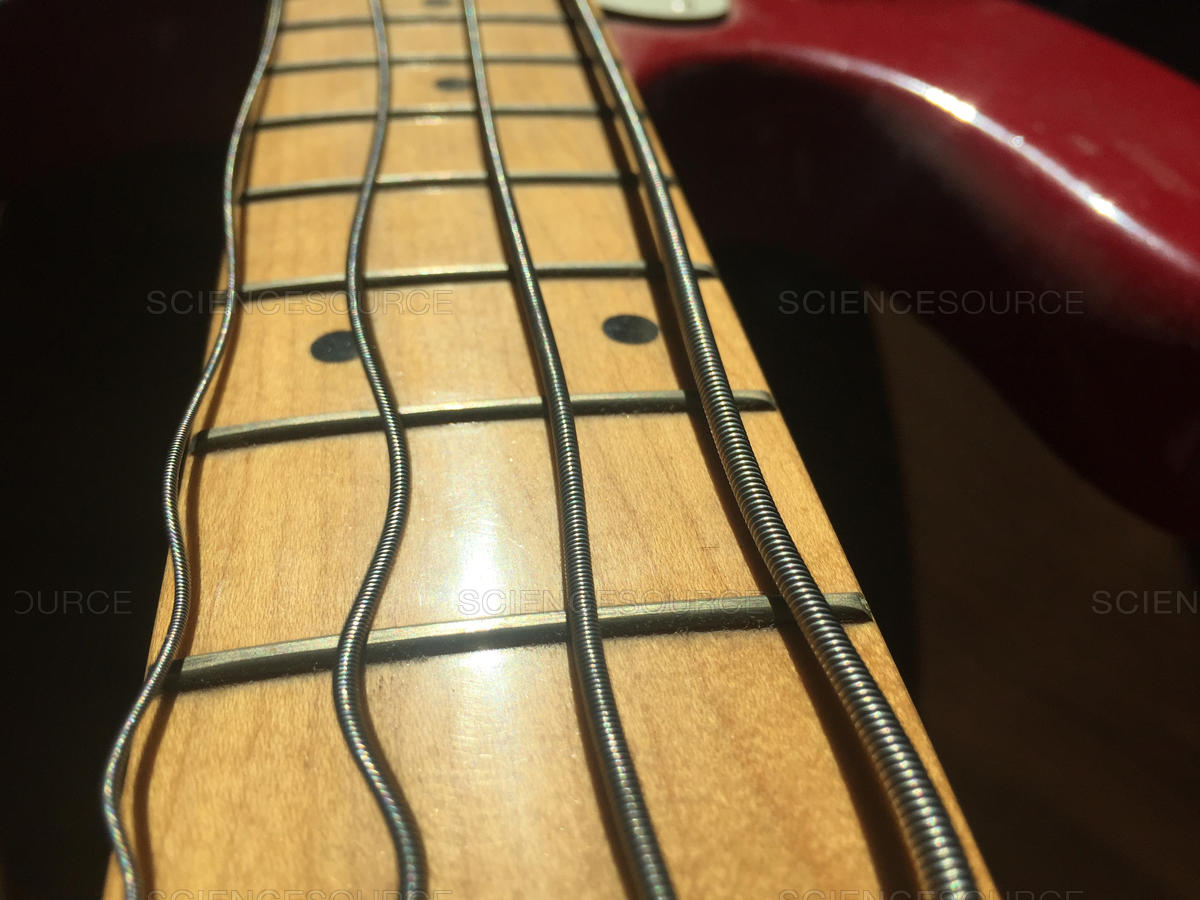
\includegraphics[scale=0.125]{stringvibration} & 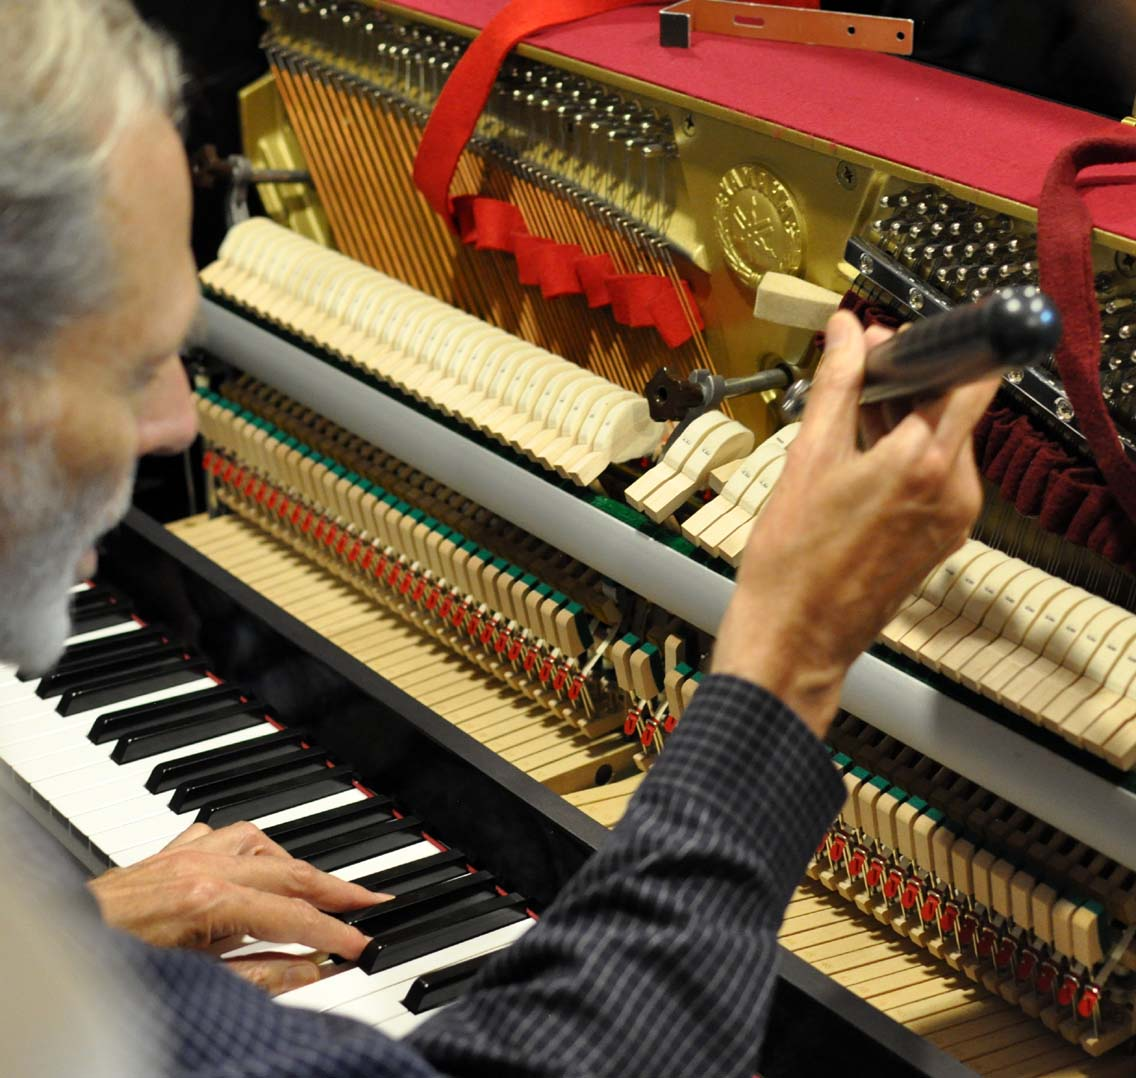
\includegraphics[scale=0.290]{pianotuning}
                \end{tabular}
            \end{center}
        \end{frame}
        \subsection{Pythagorean tunning}
        \begin{frame}
            \frametitle{Pythagorean tuning}
            \begin{center}
                Pythagorean fractions:
                $$f = \frac{i + 1}{i} ;\ i = 1, 2, ..., n$$ \\
                \vspace{1cm}
                The Pythagorean string separation:\\
                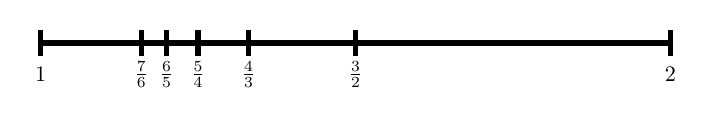
\begin{tikzpicture}[thick,scale=0.8, every node/.style={scale=0.8}]
                    \draw [line width = 2] (0, 0) -- (10, 0);
                    \draw [line width = 2] (0, 0.2) -- (0, -0.2);
                    \draw (0, -0.5)node {$1$};
                    \draw [line width = 2] (10, 0.2) -- (10, -0.2);
                    \draw (10, -0.5)node {$2$};
                    \draw [line width = 2] (5, 0.2) -- (5, -0.2);
                    \draw (5, -0.5)node {$\frac{3}{2}$};
                    \draw [line width = 2] (3.3, 0.2) -- (3.3, -0.2);
                    \draw (3.3, -0.5)node {$\frac{4}{3}$};
                    \draw [line width = 2] (2.5, 0.2) -- (2.5, -0.2);
                    \draw (2.5, -0.5)node {$\frac{5}{4}$};
                    \draw [line width = 2] (2, 0.2) -- (2, -0.2);
                    \draw (2, -0.5)node {$\frac{6}{5}$};
                    \draw [line width = 2] (1.6, 0.2) -- (1.6, -0.2);
                    \draw (1.6, -0.5)node {$\frac{7}{6}$};
                \end{tikzpicture}
            \end{center}
        \end{frame}
        \subsection{Equal temperment and 12-TET}
        \begin{frame}
            \frametitle{Equal temperment and 12-TET}
                \begin{center}
                    
                    {\tiny \begin{tabular}{| l | l | l | l |}
                        \hline
                        \textbf{Name} & \textbf{12-TET} & \textbf{Pythagorean scale}\\\hline
                        Unision ($C$) & $2^\frac{0}{12} = 1$ & $\frac{1}{1} = 1$ \\ \hline
                        Minor second ($C\sharp/D\flat$) & $2^\frac{1}{12} \approx 1.05946$ & $\frac{16}{15} \approx 1.06666$\\ \hline
                        Major second ($D$) & $2^\frac{2}{12} \approx 1.12246$ & $\frac{9}{8} = 1.125$ \\ \hline
                        Minor third ($D\sharp/E\flat$) & $2^\frac{3}{12} \approx 1.18920$ & $\frac{6}{5} = 1.2$ \\ \hline
                        Major third ($E$) & $2^\frac{4}{12} \approx 1.25992$ & $\frac{5}{4} = 1.25$ \\ \hline
                        Perfect fourth ($F$) & $2^\frac{5}{12} \approx 1.33484$ & $\frac{4}{3} \approx 1.33333$ \\ \hline
                        Tritone ($F\sharp/G\flat$) & $2^\frac{6}{12} \approx 1.41421$ & $\frac{7}{5} = 1.4$* \\ \hline
                        Perfect fifth ($G$) & $2^\frac{7}{12} \approx 1.49830$ & $\frac{3}{2} = 1.5$ \\ \hline
                        Minor sixth ($G\sharp/A\flat$) & $2^\frac{8}{12} \approx 1.58740$ & $\frac{8}{5} = 1.6$* \\ \hline
                        Major sixth ($A$) & $2^\frac{9}{12} \approx 1.68179$ & $\frac{5}{3} \approx 1.66666$* \\ \hline
                        Minor seventh ($A\sharp/B\flat$) & $2^\frac{10}{12} \approx 1.78179$ & $\frac{16}{9} \approx 1.77777$* \\ \hline
                        Major seventh ($B$) & $2^\frac{11}{12} \approx 1.88774$ & $\frac{15}{8} = 1.875$* \\ \hline
                        Octave ($C$) & $2^\frac{12}{12} = 2$ & $\frac{2}{1} = 2$ \\ \hline
                        \multicolumn{3}{c}{Note: the values with * can't be represented like Pythagorean fractions with}\\
                        \multicolumn{3}{c}{decent accuracy but the human ear can't differentiate this (in the most cases)}\\
                    \end{tabular}
                    }
                \end{center}
        \end{frame}
    \section{MIDI}
        \begin{frame}
            \frametitle{MIDI}
            MIDI is an acronym to ``Musical Instrument Digital Interface''. It:
            \begin{itemize}
                \item Developed by MIDI Manufacturers Association
                \item Targets compact representation
                \item Splited into chunks
            \end{itemize}
            This makes MIDI a perfect way to store musical data in form of notes that enables easy manipulation\\
            \begin{center}
                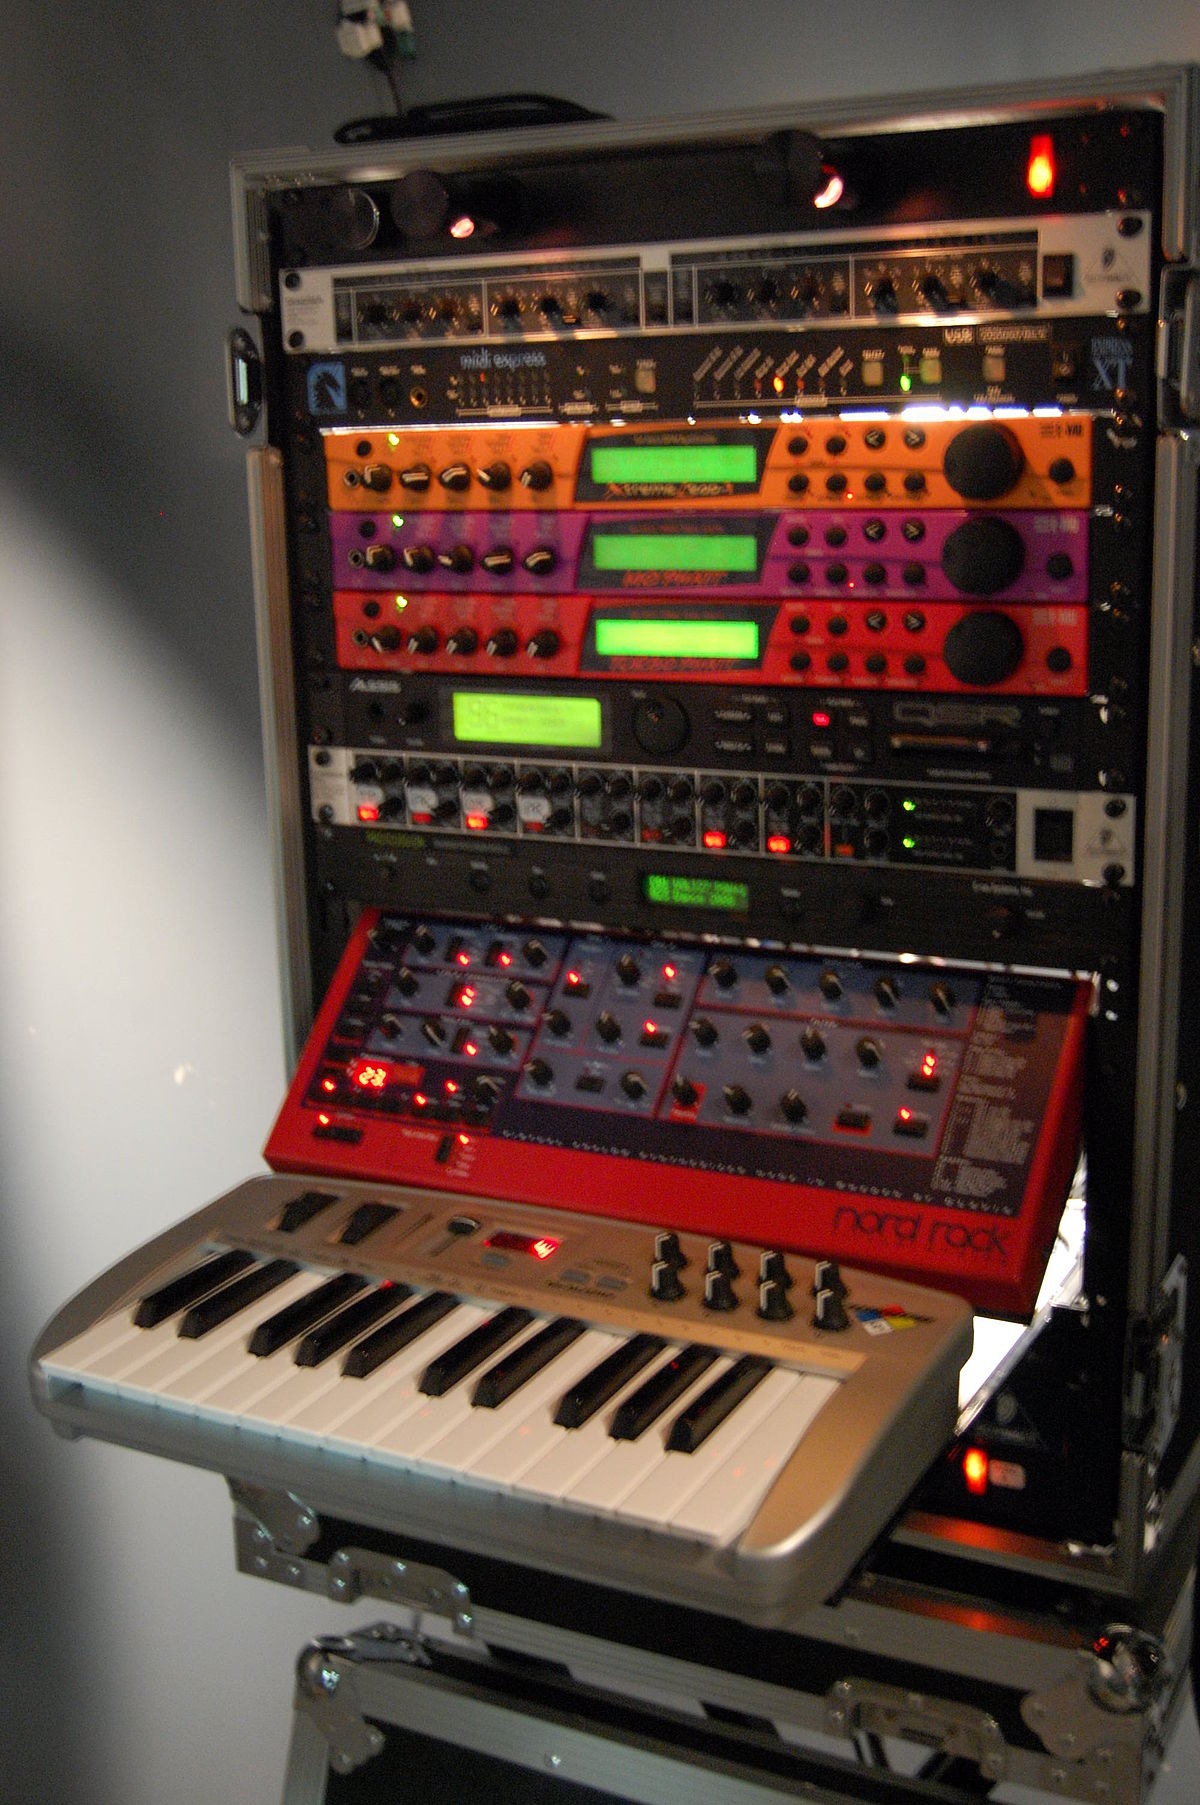
\includegraphics[scale=0.04]{midi}\hspace{1cm}
                
\includegraphics[scale=0.3]{midiasoc}
            \end{center}
            
        \end{frame}
        \subsection{Header chunk}
        \begin{frame}
            \frametitle{Header chunk}
            \begin{itemize}
                \item Contains data about the file
                \item Always one
            \end{itemize}
            \begin{center}
                {\large (M)(T)(h)(d) (0)(0)(0)(6) (0)(f) (n)(n) (d)(d)} \\ \vspace{0.5cm}
                f - the file type\\
                nn - the number of track chunks\\
                dd - the way of division of the time\\
            \end{center}
        \end{frame}
        \subsection{Track chunks}
        \begin{frame}
            \frametitle{Track chunks}
            Each track chunk is built up by events (messages). Each event has delta time and data bytes.
            The most important events are:
            \begin{itemize}
                \item NOTE\_ON - start playing a note
                \item NOTE\_OFF - stop playing a note
            \end{itemize}
            The events described above have common structure:\\
            (type;channel) (note number) (velocity)
            $$note\ number = 69 + 12\log_2 \frac{f}{440}\ where\ f\ is\ the\ frequency$$
        \end{frame}
    \section{Markov chains}
        \begin{frame}
            \frametitle{Markov chains}
            \begin{center}
                \begin{tabular}{l r}
                    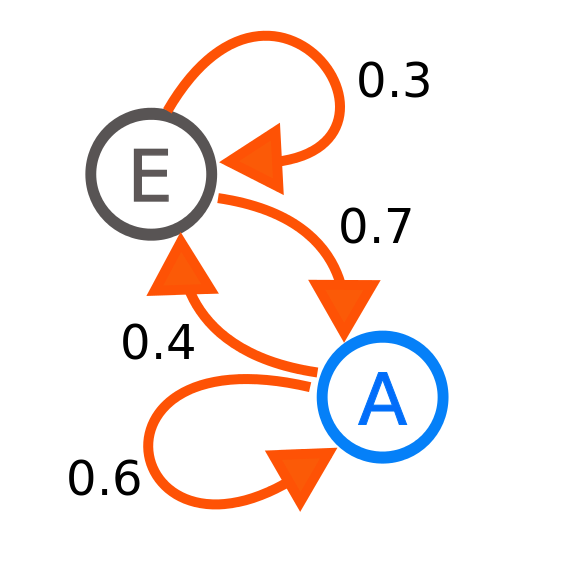
\includegraphics[scale=0.2]{mkchain} & 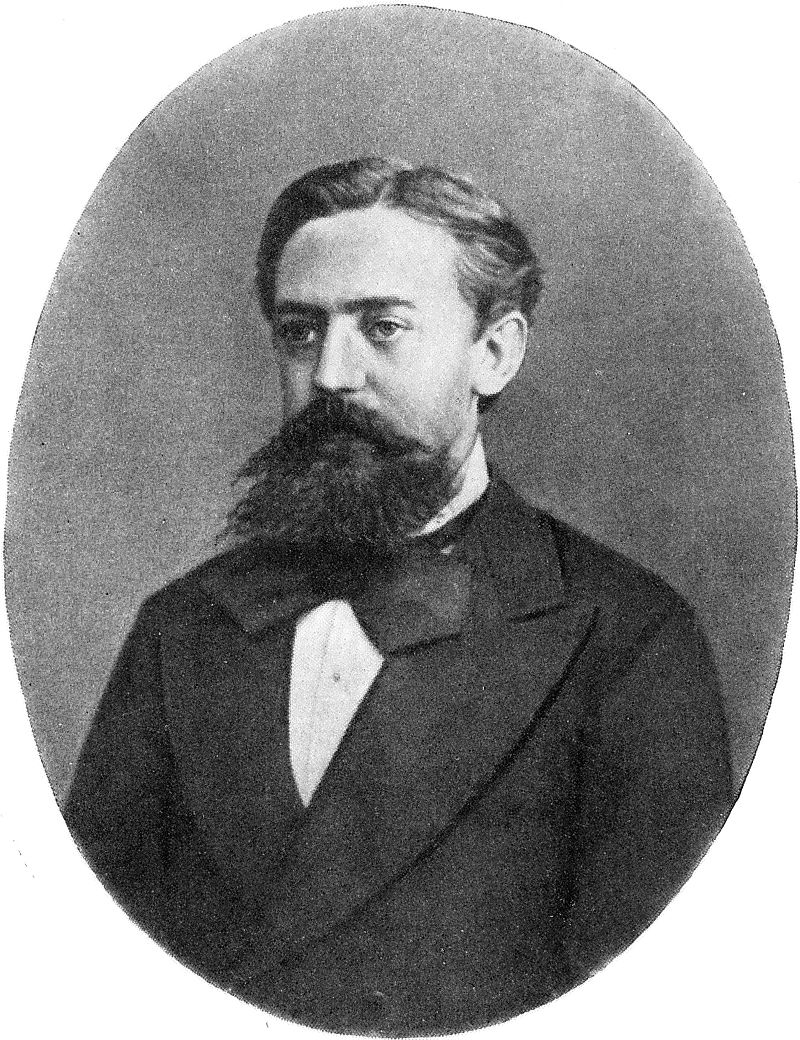
\includegraphics[scale=0.1]{markov} \\
                    Markov chain diagram & Andrey Markov
                \end{tabular}
            \end{center}
        \end{frame}
        \begin{frame}
            \frametitle{Markov chains}
            \begin{tabular}{|c|c|c|c|}
                \hline
                & \multicolumn{3}{|c|}{Next event} \\ \cline{2-4}
                & A & B & C \\ \hline
                A & 33\% & 22\% & 45\% \\ \hline
                B & 81\% & 9\% & 10\% \\ \hline
                C & 30\% & 60\% & 10\% \\ \hline
            \end{tabular}
            \begin{tabular}{|c|c|c|c|c|}
                \hline
                \multicolumn{2}{|c|}{} & \multicolumn{3}{|c|}{Next event} \\ \cline{3-5}
                \multicolumn{2}{|c|}{} & A & B & C \\ \hline
                A & A & 16\% & 16\% & 68\% \\ \hline
                A & B & 100\% & 0\% & 0\% \\ \hline
                A & C & 12\% & 75\% & 13\% \\ \hline
                B & A & 37\% & 25\% & 38\% \\ \hline
                B & B & 0\% & 0\% & 100\% \\ \hline
                B & C & 100\% & 0\% & 0\% \\ \hline
                C & A & 33\% & 33\% & 34\% \\ \hline
                C & B & 83\% & 17\% & 0\% \\ \hline
                C & C & 100\% & 0\% & 0\% \\ \hline
            \end{tabular}\\
            Example Markov chains for the string \\``AABAACBABACBABACCACAACBAAACBACBBCABAACBA''
        \end{frame}
        \section{Tested algorithms}
        \subsection{Common}
            \begin{frame}
                \frametitle{Common block diagram}
                \begin{center}
                    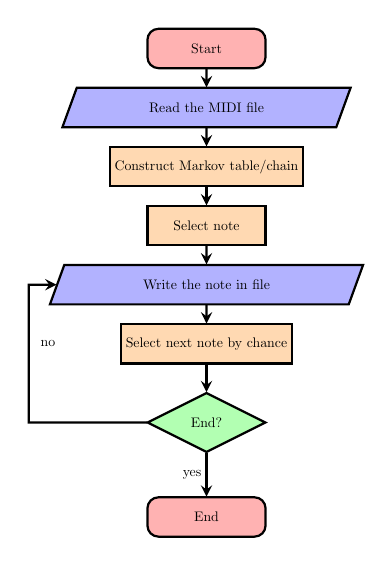
\begin{tikzpicture}[thick,scale=0.5, every node/.style={scale=0.5}, node distance=1.5cm]
                        \node (start) [startstop] {Start};
                        \node (in1) [io, below of=start] {Read the MIDI file};
                        \draw [arrow] (start) -- (in1);
                        \node (pro1) [process, below of=in1] {Construct Markov table/chain};
                        \draw [arrow] (in1) -- (pro1);
                        \node (pro2) [process, below of=pro1] {Select note};
                        \draw [arrow] (pro1) -- (pro2);
                        \node (out1) [io, below of=pro2] {Write the note in file};
                        \draw [arrow] (pro2) -- (out1);
                        \node (pro3) [process, below of=out1] {Select next note by chance};
                        \draw [arrow] (out1) -- (pro3);
                        \node (loop) [decision, below of=pro3, yshift=-0.5cm] {End?};
                        \draw [arrow] (pro3) -- (loop);
                        \draw [arrow] (loop.west) -- ++(-3,0) -- ++(0,1.75) -- ++(0,1.75) -- node[xshift=1.2cm,yshift=-1.5cm, text width=2.5cm] {no}(out1.west);
                        \node (end) [startstop, below of=loop, yshift=-0.9cm]{End};
                        \draw [arrow] (loop) -- node[anchor=east] {yes} (end);
                    \end{tikzpicture}
                \end{center}
            \end{frame}
            \subsection{Different}
            \begin{frame}
                \frametitle{Diffrences between the algorithms}
                \begin{itemize}
                    \item First algorithm - uses only the pitch of the previous note for constructing Markov chain table
                    \item Second algorithm - uses the pitch and the length of the previous note for constructing Markov chain table
                    \item Third algorithm - uses only the pitch of the previous two notes for constructing Markov chain table
                \end{itemize}
            \end{frame}
            \subsection{Results}
            \begin{frame}
                \frametitle{Results}
                
\includegraphics[scale=0.3]{notes}
            \end{frame}
            \begin{frame}
                \begin{center}
                    {\LARGE \textbf{Future development}}
                \end{center}
            \end{frame}
            \begin{frame}
                \frametitle{Questions}
                \begin{center}
                    
\includegraphics[scale=0.5]{questions}
                \end{center}
            \end{frame}
            \begin{frame}
                \begin{center}
                    {\LARGE \textbf{Thank you for the attention!}}
                \end{center}
            \end{frame}
\end{document}